\section{Evidence Response Signature}\label{sec:ers}

A risk estimator for \NDO{} verdicts can be wrong in ways that an aggregate metric such as log loss will not reveal. An estimator that lowers its risk when meaningless inputs are added, or that remains reassuring when the evidence has been tampered with, is unfit for purpose even if it happens to score well on one dataset. The Evidence Response Signature makes such requirements explicit and testable.

\subsection{Definition}
A \emph{perturbation} $T_j$ maps an evidence record to a modified copy, $\Ev \mapsto T_j(\Ev)$. For a risk estimator $\Rhat$ and decision procedure $V$, the response to $T_j$ is
\begin{equation}
\Delta_j(\Ev) \;=\; \Rhat\!\left(T_j(\Ev)\right) - \Rhat(\Ev),
\label{eq:delta}
\end{equation}
recorded together with the original and perturbed verdicts, profiles, and integrity status. The \emph{Evidence Response Signature} of $\Ev$ is the vector $\left(\Delta_j(\Ev),\, V(T_j(\Ev))\right)_{j=1}^{9}$. Each perturbation has a pre-declared expected response; a trial \emph{passes} if the observed response satisfies it, \emph{fails} if not, and is \emph{not applicable} (N/A) if the perturbation cannot be applied to $\Ev$ (for example, deleting the sole input that reaches a changed unit when no such input exists). N/A trials are never counted as passes.

\subsection{Properties}
\ers{} specifies eight properties of a reasonable false-assurance estimator, plus an environment check that the implementation adds.
\begin{enumerate}
\item \emph{Irrelevant-evidence invariance.} Adding inputs that reach no changed unit must not change the risk or the verdict.
\item \emph{Duplicate-evidence invariance.} Adding copies of existing observations must not change the risk or the verdict.
\item \emph{Relevant-evidence sensitivity.} Removing evidence that uniquely supports a changed unit must not lower the risk; the verdict may move to abstention.
\item \emph{Observation-loss sensitivity.} Removing an observation channel must not lower the risk.
\item \emph{Divergence responsiveness.} Adding an independent discriminating input must withdraw a reassuring verdict; the intended outcome is \DIV{}, and the implementation also accepts \INS{} or a risk increase.
\item \emph{Provenance sensitivity.} Degrading the provenance of the evidence must not lower the risk.
\item \emph{Evidence-integrity sensitivity.} An integrity violation must force \INS{}, irrespective of the original verdict.
\item \emph{Reproducibility sensitivity.} Reducing determinism or the repetition budget must not lower the risk.
\end{enumerate}
The additional check, \emph{environment sensitivity}, requires that marking the execution environment inconsistent must not lower the risk.

Properties 1 and 2 are invariances: they encode the principle that evidence \emph{quantity} is not evidence \emph{quality}. Properties 3, 4, 6 and 8 and the environment check are monotonicity requirements. Property 7 prescribes an exact outcome; Property 5 prescribes withdrawal of \NDO{}. The monotone properties count a move to abstention as a pass, because a procedure that withdraws a reassuring verdict when its evidence weakens is behaving correctly even if its numeric risk does not change.

\subsection{Perturbations P1--P9}
Table~\ref{tab:perturb} defines the nine perturbations and Fig.~\ref{fig:taxonomy} maps them to properties and control types. P2 and P3 are \emph{negative controls}: a correct estimator must not respond. P6 and P8 are \emph{positive controls}: a correct procedure must respond in a prescribed way. The remaining perturbations are \emph{robustness tests} of the monotone properties. P1 has a named variant, P1b, that deletes all clean inputs covering the least-multiplicity unit; it is reported with P1.

\begin{table}[!t]
\caption{Controlled evidence perturbations as implemented (\code{sbgv8/perturb.py}). All are applied to a copy of a recorded evidence record. Control: N = negative control, P = positive control, R = robustness (monotone).}
\label{tab:perturb}
\centering
\scriptsize
\setlength{\tabcolsep}{3pt}
\begin{tabular}{|c|L{3.9cm}|c|L{1.75cm}|}
\hline
Id & Operation & Ctrl. & Expected response \\
\hline
P1 & Delete one clean input that is the sole reacher of a changed unit or sole capturer of a channel (P1b: all covers of the least-multiplicity unit) & R & $\Delta\ge0$ or \INS{} \\
P2 & Append two \code{SAME} inputs that hit only unchanged lines, with fresh fingerprints & N & $|\Delta|\le0.02$, verdict unchanged \\
P3 & Append two copies of existing inputs, flagged as duplicates & N & $|\Delta|\le0.02$, verdict unchanged \\
P4 & Remove one captured channel from every input & R & $\Delta\ge0$ or \INS{} \\
P5 & Mark half of the deterministic \code{SAME} inputs non-deterministic; halve repeat counts & R & $\Delta\ge0$ or \INS{} \\
P6 & Append a confirmed-difference witness that hits all changed units & P & verdict $=\DIV{}$ (\INS{} or $\Delta>0$ accepted) \\
P7 & Mark the provenance of all inputs as label-derived & R & $\Delta\ge0$ or \INS{} \\
P8 & Set the integrity flag to violated & P & verdict $=\INS{}$ \\
P9 & Mark the execution environment inconsistent & R & $\Delta\ge0$ or \INS{} \\
\hline
\end{tabular}
\end{table}

\begin{figure*}[!t]
\centering
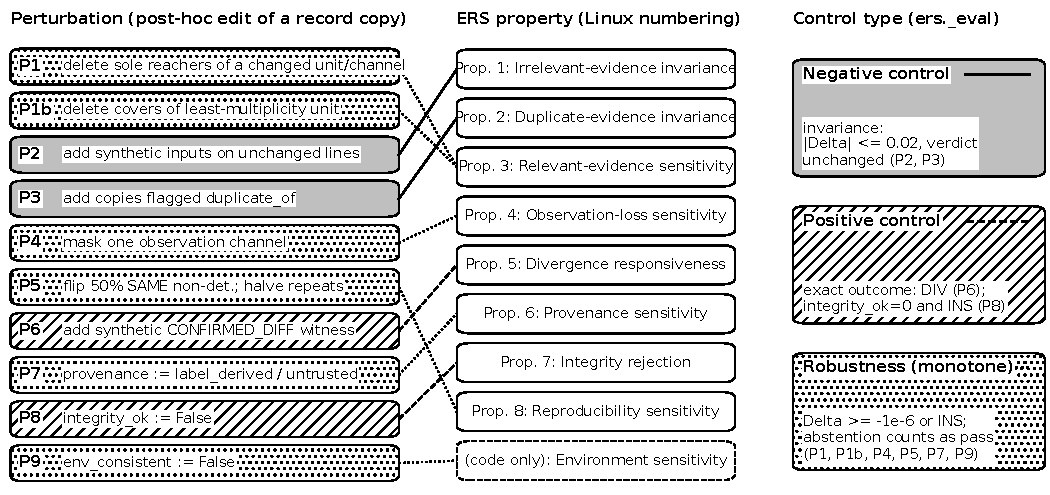
\includegraphics[width=0.86\textwidth]{figures/fig_perturbation_taxonomy.pdf}
\caption{Perturbation taxonomy. Each perturbation (left) tests one \ers{} property (centre) and is classified by the pass criterion it uses (right). P9 tests the environment check that the implementation adds to the eight properties. The tolerance $10^{-6}$ for monotone properties and $0.02$ for invariances are fixed in \code{sbgv8/ers.py}.}
\label{fig:taxonomy}
\end{figure*}

\subsection{Post-Hoc Perturbations Are Not Interventions}
All nine perturbations, as evaluated in this paper, are \emph{post-hoc transformations of recorded evidence}. They edit the record that an execution produced; they do not re-execute anything. This makes them cheap, deterministic and exactly repeatable, and it is the right instrument for testing how an \emph{estimator} responds to its input. It is the wrong instrument for estimating how a \emph{program} or a \emph{collection process} would behave under the corresponding real change. For example, P2 appends synthetic records that claim to reach only unchanged lines; a real irrelevant input could have side effects that the synthetic record does not. We therefore interpret $\Delta_j$ as a description of the estimator's behaviour, never as a causal effect of the evidence on program behaviour. A separate real-execution script for P2, P5 and P6 exists, but no raw output from it is in the replication package, and no result from it is used.

\subsection{Two Roles of the Signature}
\ers{} plays two distinct roles in \sbg{}, which must be evaluated separately.
\begin{itemize}
\item As a \emph{conformance test}, the property matrix checks whether an estimator and decision procedure satisfy the eight properties on a corpus of real evidence records. This role does not depend on labels.
\item As \emph{predictive features}, the nine responses $\Delta_j$ are appended to the profile in the full \cec{} model, on the hypothesis that how strongly an estimate reacts to evidence degradation carries information about the risk beyond the profile itself. This role is evaluated by matched-coverage risk and proper scoring rules against labelled data.
\end{itemize}
The results in Section~\ref{sec:results} support the first role and do not support the second.
